\documentclass[12pt]{article}

\usepackage[margin=1in]{geometry}
\usepackage{amsmath}
\usepackage{booktabs}
\usepackage{graphicx}
\usepackage{setspace}
\usepackage[authoryear,round]{natbib}
\setcitestyle{aysep={,}}
\usepackage{xcolor}
\usepackage{hyperref}

\doublespacing

% Items still to be verified or filled in; search for \chk before submission.
\newcommand{\chk}[1]{\textcolor{red}{\textbf{[#1]}}}

\title{Do LLM Labels Mislead Event Studies? Presidential Posts and Oil Prices}
\author{\chk{Given-name Family-name}$^{a,*}$, \chk{Given-name Family-name}$^{b}$\\[1em]
\small $^{a}$\chk{Department, University, Postal address, Country}\\
\small $^{b}$\chk{Department, University, Postal address, Country}\\[0.5em]
\small $^{*}$Corresponding author. E-mail: \chk{institutional e-mail address}}
\date{}

\begin{document}
\maketitle

\begin{abstract}
\noindent Event studies increasingly rely on large language models (LLMs) to classify news and social media posts, and the reliability of these labels is often judged by how well repeated model runs agree. We examine 191 posts by the U.S.\ president during the 2026 closure of the Strait of Hormuz, matched to tick-level oil prices. Five sets of LLM labels agree with one another ($\kappa = 0.69$--$0.84$) far more than with human coders ($\kappa = 0.44$--$0.49$), and they classify too many posts as escalation. As a result, every model label set understates the oil response to escalation posts. An exact decomposition traces the shortfall to de-escalation posts that the models misclassify as escalation. Design-based corrections remove the bias, but only once a third to a half of the posts have human labels.
\end{abstract}

\noindent\textbf{Keywords:} Large language models; Textual analysis; Event study; Misclassification; Measurement validity; Annotation; Oil prices

\noindent\textbf{JEL classification:} G14, C55, C81, Q41

\noindent\textbf{Word count (main text):} 2,339 words, excluding the abstract, references, tables, figures, captions and notes, declarations, acknowledgements, and appendices.

\clearpage

%======================================================================
\section{Introduction}

Text has become one of the main sources of information in empirical finance. Researchers use news and social media to predict returns and to date the events that event studies examine \citep{tetlock2007, loughran2011, loughran2016, gentzkow2019}, and text-based indices of geopolitical risk help explain movements in oil and other asset prices \citep{caldara2022}. Large language models (LLMs) are now taking over much of the classification work once done with dictionaries or by human coders \citep{ali2025}. They perform as well as or better than crowd workers on many annotation tasks \citep{gilardi2023}, and their reading of headlines carries information about subsequent returns \citep{lopezlira2026}. Yet when authors document the quality of LLM labels, the usual evidence is that repeated runs of a model, or different models, agree with each other \citep[e.g.,][]{garcia2026}. Such agreement shows that the labels are consistent. It says little about whether they match what a human reader would conclude.

This gap is especially consequential in event studies \citep{mackinlay1997}, because the labels determine which events are assigned to which class. Errors in a categorical variable are, by construction, correlated with the true category. They therefore do not simply attenuate an effect by a constant factor, as classical measurement error would; instead, the bias in a class mean depends on where the misclassified events come from, and it can go in either direction \citep{aigner1973, bound2001, mahajan2006, lewbel2007}. More generally, variables generated by machine learning bias downstream estimates unless they are corrected with a validated subsample \citep{yang2018, angelopoulos2023, egami2023}.

We study the problem in a setting where its consequences are easy to see. Posts by the U.S.\ president are known to move asset prices \citep{born2017, ge2019}. We examine those made during the 2026 closure of the Strait of Hormuz and link them to tick-level oil prices. An event study based on LLM labels initially suggested that oil reacted to de-escalation posts but not to escalation posts. When we compared the model labels with those of human coders, the picture changed. The model runs agree with one another at $\kappa = 0.69$ to $0.84$, but with the human coders at only $\kappa = 0.44$ to $0.49$, and they classify far too many posts as escalation, even when given the coders' own codebook. Under the human labels, oil moves in the implied direction after both types of post. Every set of model labels understates the response to escalation, although with only ten human-labelled escalation events this shortfall is not statistically significant.

The paper contributes to the growing use of LLM labels in finance in three ways. First, it documents a case in which consistency and validity diverge sharply. Second, it expresses the model-label event-study estimate as an exact weighted average of human-class means. This decomposition shows that the shortfall arises because de-escalation posts are misclassified as escalation, and not because correctly labelled posts elicit a weaker response. Third, it shows that design-based corrections, at the scale of a typical event study, require human labels for a third to a half of the events before they improve accuracy. We do not claim that the posts caused the price movements; the market response serves only to make the consequences of the labelling visible.

%======================================================================
\section{Case and Data}

\subsection{Posts}
The war with Iran began on February 28, 2026, and the strait was effectively closed from early March. CNN's archive of the president's posts contains 4,838 original posts between March 1 and October 13, 2026. From these, a keyword search yields a frame of 191 war-period posts about Iran and the strait. Each post is assigned to one of four classes: escalation, de-escalation, mixed (a clear threat combined with a clear pause or concession), or other.

\subsection{Model labels}
The original labels come from two runs of claude-sonnet-5-5 that saw only the text of each post, used default sampling settings, and had no codebook. We use the first run (``model~1''). After the human validation, four further runs (claude-opus-5-5, claude-haiku-5-5, and two runs of claude-sonnet-5-5) relabelled all posts. These runs received only the human coders' codebook (v2) and the post texts. We refer to their modal label as the ``v2 majority.'' Prompts and execution details are given in Appendix A.

\subsection{Human labels}
Two doctoral students in information systems, who knew neither the research question nor the market data, labelled all 191 posts using codebook v2. Their agreement is $\kappa = 0.67$ \citep{cohen1960}, and they disagreed on 45 posts. To keep the investigator out of the final labels, an independent third coder resolved these disagreements, following a plan committed in advance. On 15 unmarked control posts, this coder agreed with the original consensus at $\kappa = 0.45$. The final labels comprise 83 other, 46 de-escalation, 34 mixed, and 28 escalation posts. We regard them as a benchmark rather than as the truth, because agreement among the coders is only moderate and all of them remembered how the war unfolded.

\subsection{Outcome}
The outcome is the log return on a West Texas Intermediate (WTI) crude contract for difference, measured from the last tick before a post to 30 minutes after it and signed in the direction that the post implies. Given the short window, we use raw rather than abnormal returns. Posts made within three hours of another post, or while the market was closed, are excluded. This leaves 95 events, and every label set is evaluated on the same events. Inference relies on Wilcoxon tests and a bootstrap clustered by day. Appendix F provides further details, and Appendix G reports the status of each analysis.

%======================================================================
\section{Consistency Is Not Validity}

Judged by the criterion most often reported, the model labels look reliable. The two original runs agree at $\kappa = 0.74$, and the four codebook-v2 runs at $\kappa = 0.69$ to $0.84$. The models thus agree with each other at least as well as the two human coders do (Table 1, Panel A).

Agreement with the human labels is much weaker (Panel B), at $\kappa = 0.44$ to 0.49. Gwet's AC1, which is robust to the large share of posts in the ``other'' class \citep{gwet2008}, yields almost identical values. Most of the disagreement concerns a single class. The human coders assign 28 posts to escalation, whereas the model runs assign between 63 and 85. Escalation precision is consequently only 0.29 to 0.35, while recall is 0.79 to 0.93. In other words, the models seldom miss a post that humans regard as escalation, but they add many that humans do not.

One might object that the original model never saw the codebook. Before running the v2 models, we therefore set a threshold: the gap would be attributed to the prompt if the new runs reached $\kappa \geq 0.60$ and an escalation precision of at least 0.70. None comes close. The most direct test is provided by the two claude-sonnet-5-5 runs, which differ from the original only in the prompt. Their agreement with the human coders is $\kappa = 0.44$ and 0.45, compared with 0.48 for the original run. Agreement between runs, then, shows that a model gives the same answer twice. It does not show that the answer is the one a human reader would give.

\begin{center}[Insert Table 1 about here]\end{center}

%======================================================================
\section{Labels Change the Event-Study Estimate}

Since every label set is applied to the same 95 events, differences between the estimates reflect only how each set allocates events to classes (Figure 1). For de-escalation, the choice of labels hardly matters. The 30-minute response ranges from 0.90\% to 1.04\% across label sets, compared with 0.94\% under the human labels ($n = 32$; Wilcoxon $p = 0.0003$). For escalation, every model label set produces a smaller estimate, between 0.17\% and 0.35\%, compared with 0.45\% under the human labels ($n = 10$; $p = 0.084$; CI 0.02 to 0.89).

This pattern accounts for the original one-sided result. With model~1 labels, the escalation response is indistinguishable from zero (0.17\%, $p = 0.53$), whereas with the v2 majority it is 0.32\% ($p = 0.047$). Whether escalation posts appear to ``matter'' thus depends on which model run the researcher happens to use.

With only ten human-labelled escalation events, none of the differences between the human and model estimates is statistically significant. The largest, for model~1, is 0.28 percentage points (95\% CI $-0.07$ to 0.69), and the difference between a significant and an insignificant estimate is not itself a test \citep{gelman2006}. The human escalation estimate is also sensitive to a few events (Table F.2). The evidence is better described as a consistent pattern. The shortfall has the same sign under all five model label sets, and the de-escalation estimate is unaffected. This suggests that the models systematically place the wrong kind of post in the escalation class.

\begin{center}[Insert Figure 1 about here]\end{center}

%======================================================================
\section{A Misclassification Decomposition}

Because the model and human labels refer to the same events, the model-label estimate can be expressed exactly in terms of the human classes. Let $H$ be the human label of an event, $M$ a model label, and $r_e$ the return signed in the direction of class $e$. The model-label estimate can then be written as
\begin{equation}
\mu_M(e) \;=\; \sum_{h} \pi(h \mid e)\,\mu(h, e),
\label{eq:mixture}
\end{equation}
where $\pi(h \mid e)$ is the share of events in model class $e$ that humans assign to class $h$, so that $\pi(e \mid e)$ is the precision, and $\mu(h, e)$ is the mean of $r_e$ over these events. Subtracting the human estimate $\mu_H(e)$ yields
\begin{equation}
\mu_M(e) - \mu_H(e) \;=\; \underbrace{\pi(e \mid e)\,\big[\mu(e, e) - \mu_H(e)\big]}_{\text{selection within the class}} \;+\; \underbrace{\sum_{h \neq e} \pi(h \mid e)\,\big[\mu(h, e) - \mu_H(e)\big]}_{\text{contamination}}.
\label{eq:gap}
\end{equation}
Equation~(1) is an accounting identity and requires no assumptions about how the errors arise. It does, however, make concrete the econometric result that misclassification bias is a weighted sum of differences in outcomes between classes \citep{aigner1973, mahajan2006, lewbel2007}.

Table 2 reports each term for the escalation class. For model~1, the gap of $-0.28$ percentage points consists of $+0.02$ from selection within the class, $-0.24$ from posts that humans classify as de-escalation, $+0.02$ from mixed posts, and $-0.08$ from posts in the other class. For the v2 majority, the corresponding figures for a gap of $-0.13$ are 0.00, $-0.16$, $+0.09$, and $-0.06$.

First, the shortfall does not stem from a weaker reaction to correctly labelled posts. Events that both humans and models classify as escalation move oil by 0.52\% and 0.44\%, close to the 0.45\% for the human class as a whole.

Second, most of the bias comes from de-escalation posts that the models place in the escalation class. Six of model~1's 24 escalation events are de-escalation posts in the human coders' judgment. Signed as escalation, their return is $-0.51$\%. Such a post does more harm to the estimate than an unrelated post, whose contribution is close to zero.

Third, precision is a poor guide to bias. On these events the v2 majority is slightly less precise than model~1 (9 of 30, compared with 8 of 24), yet its bias is less than half as large. The reason is that its errors come from different classes. Most of the posts it adds are mixed posts, which humans also read as containing a threat and which move oil in the escalation direction ($+0.68$\%), and fewer are de-escalation posts (4 compared with 6). Two label sets with similar $\kappa$ and precision can therefore bias an estimate by quite different amounts.

The same identity explains why the de-escalation estimate is stable: precision is higher, and no post that humans regard as escalation enters the class (Table D.1). Since each term can be estimated on any validated subsample, the decomposition can also serve as a diagnostic in applied event studies. It is, however, defined relative to human labels that are themselves measured with error, and so it does not recover the true response. With several raters per post, a latent-class extension would be identified under conditions on how the raters' errors are related \citep{hu2008}. We note that the decomposition was formulated after the event-level results were known (post hoc; Appendix G).

\begin{center}[Insert Table 2 about here]\end{center}

%======================================================================
\section{How Much Validation Is Enough?}

Prediction-powered inference \citep{angelopoulos2023} and design-based supervised learning \citep[DSL;][]{egami2023} correct model-label estimates using human labels for a random subsample. We ran an exploratory simulation in which 10\% to 50\% of the posts were validated (Appendix E). DSL removed the bias, but with only ten escalation events it outperformed the naive model-label estimate only once about 30\% of posts had been validated under the model~1 labels. With the more accurate v2 majority labels, even validating 50\% was not sufficient. When events are few, a validated subsample is not a cheap remedy.

%======================================================================
\section{Recommendations and Limits}

Based on this case, we suggest four practices for event studies that rely on LLM labels.

\begin{enumerate}
\item \textbf{Report validity by class, not only consistency.} Agreement between runs should be presented as evidence of reliability. Agreement with human coders should be reported for each class, using a prevalence-robust measure alongside $\kappa$, together with precision and recall for the classes analysed.
\item \textbf{Give models and human coders the same instructions.} Authors should state who wrote the codebook, when, and with what knowledge of earlier errors.
\item \textbf{Compare and decompose.} The event response should be estimated under alternative label sets on the same events, and any difference decomposed using equation~(2).
\item \textbf{Check whether a correction pays off at the available sample size}, by simulating it on the validated subsample.
\end{enumerate}

The evidence has clear limitations. It comes from a single episode, a single sender, and a single asset, and the escalation result rests on ten events. Half of the escalation posts that signal a direction were made while the market was closed and are therefore lost, compared with 18\% of the de-escalation posts. The human labels provide a moderately reliable benchmark, formed with the benefit of hindsight. We tested one family of models, under default settings, in one commodity market. Finally, the decomposition and the simulation were designed after the main results were known, and the event sample was redefined as the quality of the labels became clear; Online Appendix G documents each version.

Had we reported only the agreement between model runs, we would have endorsed labels that changed the answer. Before a set of labels is used to define the events in an event study, the relevant evidence is its agreement with human readers, not its agreement with itself.

\clearpage
\section*{Declarations}

\subsection*{Data availability}
\chk{Replication code, prompts, model outputs, coder sheets, and analysis plans will be deposited in a public repository (for example, Mendeley Data) on acceptance. Post texts come from a public archive; tick data are from Dukascopy (check redistribution terms).}

\subsection*{Declaration of generative AI and AI-assisted technologies in the writing process}
Large language models were used as classification instruments, as described in Section~2 and the Online Appendix. \chk{State any use of generative AI in writing or coding, following the journal's required wording.}

\subsection*{Ethics}
\chk{State whether ethics approval was required for the human coding (e.g., exempt or not applicable), following your institution's rules.}

\subsection*{Declaration of competing interest}
\chk{The authors declare no competing interests.}

\subsection*{Funding}
\chk{Funding statement, or ``This research did not receive any specific grant from funding agencies in the public, commercial, or not-for-profit sectors.''}

\subsection*{CRediT authorship contribution statement}
\chk{Author contributions.}

\section*{Acknowledgements}
\chk{Acknowledgements, including any help with language, writing, or proofreading.}

\bibliographystyle{plainnat}
\bibliography{references}

\clearpage
\section*{Tables and figures}

\begin{table}[p]
\centering
\small
\caption{Consistency Between Runs and Validity Against Human Coders}
\label{tab:agreement}
\begin{tabular}{lcc}
\multicolumn{3}{l}{\textit{Panel A. Consistency (agreement between raters of the same kind)}}\\
\toprule
Comparison & Posts & $\kappa$ \\
\midrule
Model 1 vs.\ its second run (claude-sonnet-5-5, no codebook)$^{a}$ & 150 & 0.74 \\
Four codebook-v2 runs, six pairwise comparisons & 191 & 0.69--0.84 \\
Human coder 1 vs.\ human coder 2 (codebook v2) & 191 & 0.67 \\
\bottomrule
\end{tabular}

\vspace{1em}
\begin{tabular}{lllcccc}
\multicolumn{7}{l}{\textit{Panel B. Validity (agreement with the final human labels, 191 posts)}}\\
\toprule
Label set & Codebook & $\kappa$ (95\% CI) & AC1 & Esc.\ labels & Esc.\ P / R & De-esc.\ P / R \\
\midrule
Model 1 (sonnet) & none & 0.48 (0.39--0.56) & 0.50 & 63 & 0.35 / 0.79 & 0.63 / 0.78 \\
v2 opus & v2 & 0.47 (0.39--0.55) & 0.48 & 78 & 0.32 / 0.89 & 0.70 / 0.80 \\
v2 sonnet & v2 & 0.44 (0.37--0.53) & 0.45 & 85 & 0.29 / 0.89 & 0.76 / 0.74 \\
v2 haiku & v2 & 0.49 (0.40--0.57) & 0.50 & 76 & 0.34 / 0.93 & 0.77 / 0.74 \\
v2 sonnet repeat & v2 & 0.45 (0.36--0.53) & 0.45 & 73 & 0.34 / 0.89 & 0.70 / 0.70 \\
v2 majority & v2 & 0.49 (0.42--0.58) & 0.50 & 77 & 0.32 / 0.89 & 0.73 / 0.80 \\
\bottomrule
\end{tabular}

\vspace{0.5em}
\begin{minipage}{0.95\textwidth}
\footnotesize\textit{Note:} $^{a}$Computed on the first-round validation sample (150 posts, including pre-war and other oil-related posts), not on the 191-post frame. The final human labels assign 28 posts to escalation and 46 to de-escalation. P / R = precision / recall. Model 1: original labels from claude-sonnet-5-5 given only the post text. v2 runs: re-labelling given the human coders' codebook (v2); v2 majority: their modal label. AC1 is Gwet's prevalence-robust agreement coefficient.
\end{minipage}
\end{table}

\clearpage
\begin{figure}[p]
\centering
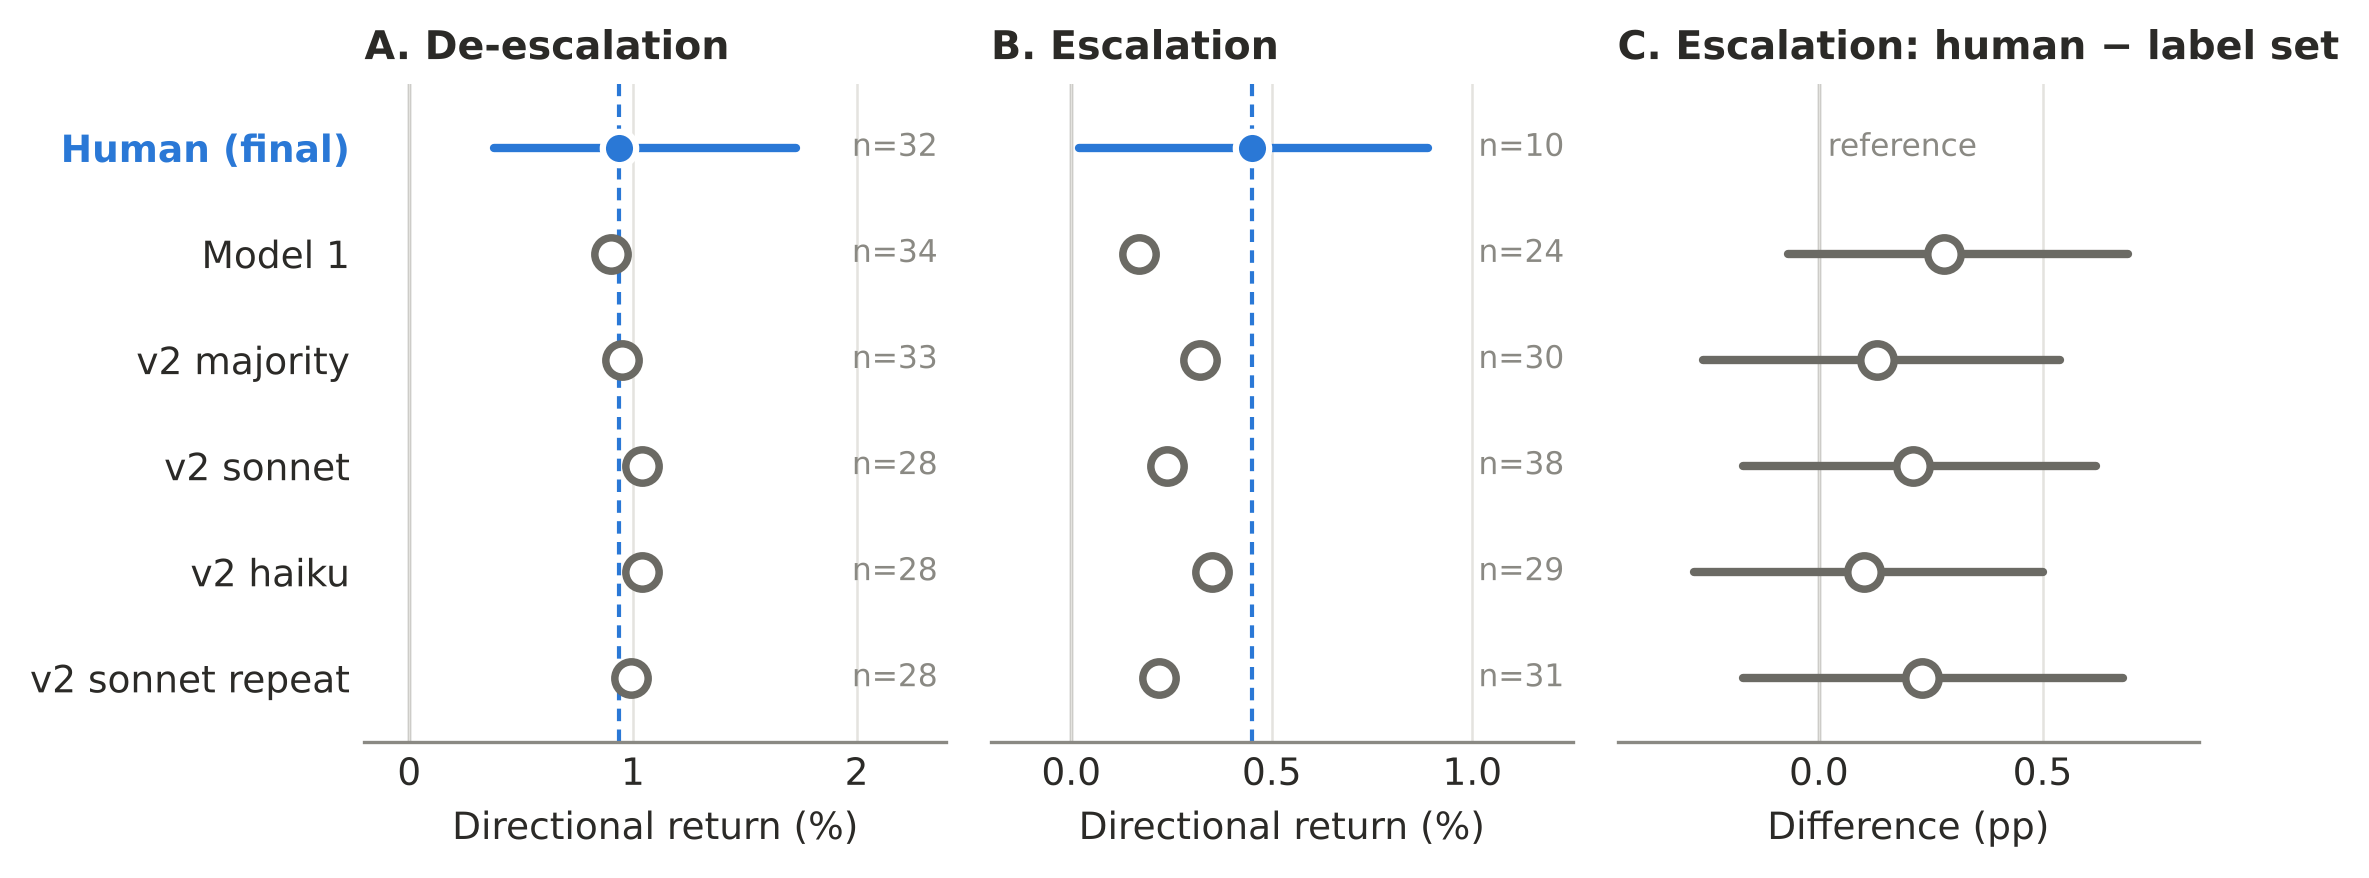
\includegraphics[width=\textwidth]{Figure_1.png}
\caption{Mean Directional 30-Minute WTI Return by Class Under Each Label Set}
\label{fig:labelsets}
\begin{minipage}{0.95\textwidth}
\footnotesize\textit{Note:} The same 95 events under every label set. Panels A and B: points are mean 30-minute returns signed in the direction of the class; the bar on the human row is its day-clustered bootstrap 95\% confidence interval, and the dashed line marks the human estimate. Numbers at the right give the events in each class. Panel C: human minus label-set escalation estimate, with day-clustered bootstrap 95\% confidence intervals (10,000 resamples). The v2 opus run gives the same results as the v2 majority. Label sets as defined in Table 1. The figure was drawn in Python from the estimates in Online Appendix Table C.1, with plotting code written with the assistance of a generative AI tool.
\end{minipage}
\end{figure}

\clearpage
\begin{table}[p]
\centering
\small
\caption{Misclassification Decomposition of the Escalation Estimate}
\label{tab:decomp}
\begin{tabular}{lcc}
\toprule
 & Model 1 & v2 majority \\
\midrule
Model-labelled escalation events & 24 & 30 \\
\quad Human escalation (same class) & 8 ($+0.52$) & 9 ($+0.44$) \\
\quad Human de-escalation & 6 ($-0.51$) & 4 ($-0.75$) \\
\quad Human mixed & 7 ($+0.52$) & 12 ($+0.68$) \\
\quad Human other & 3 ($-0.21$) & 5 ($+0.09$) \\
\midrule
Mean, eq.~(1) & $+0.17$ & $+0.32$ \\
Human estimate $\mu_H(e)$ & $+0.45$ & $+0.45$ \\
\textbf{Gap, eq.~(2)} & $\mathbf{-0.28}$ & $\mathbf{-0.13}$ \\
\quad Selection within the class & $+0.02$ & $0.00$ \\
\quad Contamination: de-escalation & $-0.24$ & $-0.16$ \\
\quad Contamination: mixed & $+0.02$ & $+0.09$ \\
\quad Contamination: other & $-0.08$ & $-0.06$ \\
\bottomrule
\end{tabular}

\vspace{0.5em}
\begin{minipage}{0.85\textwidth}
\footnotesize\textit{Note:} Same 95-event frame. Final human labels (10 escalation events). Cells give the number of model-labelled escalation events with each human label and, in parentheses, their mean 30-minute WTI return (percent), signed in the escalation direction. Components are rounded and need not sum exactly. Model 1 and v2 majority as defined in Table 1. The decomposition for the de-escalation class is in Online Appendix Table D.1.
\end{minipage}
\end{table}

\end{document}
